\documentclass[12pt, a4paper]{article}
\usepackage[utf8]{inputenc}
\usepackage[T1]{fontenc}
\usepackage[french]{babel}
\usepackage{geometry}
\usepackage{amsmath}
\usepackage{amssymb}
\usepackage{graphicx}
\usepackage{enumitem}
\usepackage{ulem}
\usepackage{booktabs}
\usepackage{array}
\usepackage{hyperref}
\usepackage{xcolor}
\usepackage{float}
\usepackage{caption}
\usepackage{adjustbox}
\usepackage{tikz}
\usepackage{enumitem}
\usepackage{fancyhdr}
\usepackage{titlesec}
\usepackage{setspace}
\usepackage{hyperref}
\usepackage{bookmark}

 % Ajout du package pour les en-têtes

\usetikzlibrary{calc, shapes.geometric}
\geometry{margin=2cm}

% Configuration de l'en-tête
\pagestyle{fancy}
\fancyhf{} % Efface les en-têtes et pieds de page par défaut
\renewcommand{\headrulewidth}{0.4pt}
\renewcommand{\headrule}{\hrule width\headwidth height\headrulewidth}
\fancyhead[C]{\rule{\textwidth}{0.4pt}} % Ligne centrée
\fancyhead[R]{\textit{Investigation numérique}} % Texte à droite
\fancyfoot[C]{\thepage} % Numéro de page centré

% Marges réduites

\definecolor{blue1}{RGB}{0, 51, 102}
\definecolor{blue2}{RGB}{0, 102, 204}
\definecolor{gray1}{RGB}{240, 240, 240}

\geometry{margin=2.5cm}

\setlength{\parindent}{0pt}
\setlength{\parskip}{1em}



\begin{document}
	\begin{titlepage}
		
		% Bordure autour de la page
		\begin{tikzpicture}[remember picture, overlay]
			\draw[line width=2pt, black] 
			($(current page.north west) + (0.5cm,-0.5cm)$) rectangle 
			($(current page.south east) + (-0.5cm,0.5cm)$);
		\end{tikzpicture}
		
		\centering
		
		% SOLUTION FONCTIONNELLE : Tableau avec alignement en bas
		\begin{tabular}{@{}p{0.25\textwidth}@{\hspace{2cm}}c@{\hspace{0.5cm}}p{0.5\textwidth}@{}}
			% Colonne de gauche (Français) - ALIGNÉ EN BAS
			\begin{minipage}[t][5cm][b]{0.39\textwidth}
				\raggedright
				\begin{center}
					{\small \textbf{RÉPUBLIQUE DU CAMEROUN}}\\
					{\small \textbf{******}}\\
					{\small \textbf{UNIVERSITÉ DE YAOUNDÉ}}\\
					{\small \textbf{I}}\\
					{\small \textbf{******}}\\
					{\small \textbf{ÉCOLE NATIONALE SUPÉRIEURE POLYTECHNIQUE}}\\
					{\small \textbf{******}}\\
					{\small \textbf{DÉPARTEMENT DU GÉNIE INFORMATIQUE}}\\
				\end{center}
			\end{minipage}
			&
			% Colonne du centre (LOGO EN BAS)
			\begin{minipage}[t][5cm][b]{0.2\textwidth}
				\centering
				
				\vspace*{\fill} % Pousse le logo vers le bas
				
\includegraphics[width=\textwidth, height=3cm]{logo.jpeg}
				\vspace*{\fill} % Espace en bas
			\end{minipage}
			&
			% Colonne de droite (Anglais) - ALIGNÉ EN BAS
			\begin{minipage}[t][5cm][b]{0.36\textwidth}
				\raggedright
				\begin{center}
					{\small \textbf{REPUBLIC OF CAMEROON}}\\
					{\small \textbf{******}}\\
					{\small \textbf{UNIVERSITY OF YAOUNDE I}}\\
					{\small \textbf{******}}\\
					{\small \textbf{NATIONAL ADVANCED SCHOOL OF}}\\
					{\small \textbf{ENGINEERING}}\\
					{\small \textbf{******}}\\
					{\small \textbf{DEPARTMENT OF COMPUTER ENGINEERING}}\\
				\end{center}
			\end{minipage}
		\end{tabular}
		
		\vspace{1.5cm}
		
		% Ligne séparatrice
		\noindent\rule{0.9\textwidth}{0.8pt}\\
		\vspace{0.5cm}
		
		% Thème
		\vspace{0.8cm}
		{\Large \textbf{Rapport de l'investigation numérique sur mon binome}}\\
		\vspace{0.8cm}
		
		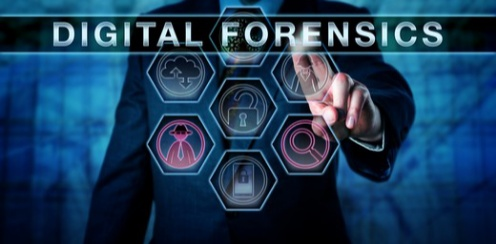
\includegraphics[width=0.5\textwidth]{For.jpeg}
		% Ligne séparatrice
		\noindent\rule{0.9\textwidth}{0.8pt}\\
		\vspace{1.5cm}
		
		% Informations étudiant
		\begin{tabular}{@{}>{\bfseries}l l@{}}
			\vspace{0.5cm}
			Réalisé par : & \textbf{NANTIA ZAGUE AXEL FRISKYL} \\
			\vspace{0.5cm}
			Matricule : & \textbf{22P105} \\
			\vspace{0.5cm}
			Spécialité : & \textbf{Cybersécurité et Investigation Numérique (CIN)} \\
			\vspace{0.5cm}
			UE : & \textbf{Introduction aux techniques de l'Investigations Numériques} \\
			\vspace{0.5cm}
			Sous la supervision de : & \textbf{Mr. MINKA MI NGUIDJOI Thierry Emmanuel} \\
			\vspace{0.5cm}
			Année académique : & \textbf{2025/2026} \\
		\end{tabular}
		
	\end{titlepage}
	
	\newpage
	
	% Table des matières
	\section*{Table des matières}
	\addcontentsline{toc}{section}{Table des matières}
	
	\begin{itemize}[leftmargin=*]
		\item \hyperref[introduction]{\textbf{Introduction}} [2]
		\item \hyperref[presentation]{\textbf{Présentations des informations que nous disposons sur MBETI avant l'investigation}} [3]
		\item \hyperref[methodologie]{\textbf{Méthodologie a suivre pour bien mené une investigation numérique sur un individu}} [4]
		\item \hyperref[resultats]{\textbf{Résultat obtenu après investigation}} [5]
		\item \hyperref[comparaison]{\textbf{Comparaison des informations probablement connues et celles trouvées}} [6]
		\item \hyperref[recommandations]{\textbf{Recommandations}} [7]
		\item \hyperref[conclusion]{\textbf{Conclusion}} [8]
	\end{itemize}
	
	\newpage
	
	
	% Introduction
	\section{\textbf{Introduction}\label{introduction}}
	
	Investigation numérique : enquête et analyse du profil numérique de mon binôme. Ce rapport individuel présente l'investigation numérique menée afin d'analyser et de traquer en ligne le profil de mon binôme MBETI DJOFANG LINDSAY AIMÉ. L'objectif principal est de confronter les informations dont je disposais initialement à celles récoltées à l'issue d'une méthodologie rigoureuse d'analyse des traces et comportements en ligne. Dans cette démarche, plusieurs étapes ont été suivies : identification et collecte d'informations sur des sources ouvertes (réseaux sociaux, moteurs de recherche, bases de données publiques), exploitation d'outils spécialisés pour extraire et analyser les données numériques accessibles publiquement, puis interprétation des résultats en vue de reconstituer un profil cohérent. Ce travail met aussi en lumière les limites inhérentes à ce type d'investigation mené dans un cadre légal et éthique strict. Le rapport s'articule en quatre grandes parties : ce que je savais déjà de MBETI DJOFANG LINDSAY AIMÉ avant l'enquête, la description précise de la méthodologie mise en œuvre pour le traquer en ligne, les résultats obtenus à l'issue de cette démarche, et enfin une comparaison critique entre les attentes initiales et les faits recueillis. Ce document a été réalisé dans le cadre du cours d'investigation numérique sous la supervision de M. MINKA.
	
	\newpage
	
	% Présentations des informations
	\section{\textbf{Présentations des informations que nous disposons sur MBETI avant l'investigation}\label{presentation}}
	
	MBETI DJOFANG LINDSAY AIMÉ est étudiante à l'École Nationale Supérieure Polytechnique de Yaoundé (Polytechnique), promotion 2027, où elle poursuit actuellement sa 4ème année en cyber sécurité et investigation numérique. Elle a débuté ses études en 2023 et a montré un intérêt marqué pour la sécurité des systèmes, le hacking éthique, ainsi qu'un certain intérêt pour le black hacking. Passionnée par les jeux d'aventure et de réflexion, les mangas, les romans et les animés, elle est décrite comme une personne objective, intelligente, sage et engagée, notamment en tant que déléguée depuis sa première année. Sur le plan académique, MBETI a commencé une formation CCNA en 2024 pour approfondir ses compétences en réseau, et elle détient deux certificats Fortinet (FCA et FCF). Elle est également reconnue pour sa performance régulière dans ses devoirs malgré quelques moments de manque de sérieux. Elle aime grignoter et fréquenter le restaurant SOS. Socialement, elle entretient de fortes relations d'amitié, notamment avec ONGUENE BELLA, Hilary et Ze. D'autres informations recueillies auprès de ses proches indiquent qu'elle a fréquenté plusieurs établissements scolaires avant Polytechnique, notamment PI AND JU et le Collège Jean Tabi. Née le 23 mai 2004 à Yaoundé 1, elle est célibataire et réside à Messassi-Nkolodom. Elle est issue d'une fratrie de trois enfants, avec un frère et une sœur, et porte les noms de ses parents ONGUENE ONGUENE Alain Roland et AKABA Romaine Émilie. Malgré ce que l'on pourrait croire, elle déclare ne pas avoir de repas préféré et ne possède pas de meilleur ami officiel. Cette connaissance préliminaire sur MBETI DJOFANG LINDSAY AIMÉ servira de base pour comparer et compléter les résultats issus de l'investigation numérique proprement dite, afin d'évaluer la cohérence et l'étendue des informations accessibles en ligne.
	
	\newpage
	
	% Méthodologie
	\section{\textbf{Méthodologie a suivre pour bien mené une investigation numérique sur un individu}\label{methodologie}}
	
	L'investigation numérique sur une personne repose sur des méthodologies rigoureuses, des techniques précises et des outils spécialisés visant à collecter, analyser et interpréter des données numériques dans le respect du cadre légal. La méthodologie comprend plusieurs étapes essentielles.
	
	\begin{enumerate}[leftmargin=*]
		\item \textbf{Identification :} Cette étape consiste à définir clairement la cible de l'investigation, c'est-à-dire la personne recherchée, et à recenser toutes les sources potentielles d'information, telles que les réseaux sociaux, les bases de données publiques, les moteurs de recherche, forums, plateformes de messagerie, et autres traces numériques accessibles. Il s'agit aussi de recueillir les informations préalables connues qui orienteront la recherche.
		
		\item \textbf{Préservation :} Une fois les informations localisées, il est essentiel de les préserver dans leur intégrité pour éviter toute altération qui compromettrait la valeur probante des données. Cette phase utilise des techniques comme la duplication bit à bit et l'emploi de dispositifs de protection en écriture.
		
		\item \textbf{Collecte et extraction des données :} Cette phase utilise des outils d'Open Source Intelligence (OSINT) pour récolter les données sur la cible, tels que Maltego, SpiderFoot, ou des scripts personnalisés. Des logiciels spécifiques permettent d'extraire les données numériques issues de différents supports (ordinateurs, téléphones, serveurs) tout en garantissant la traçabilité.
		
		\item \textbf{Analyse :} Les données collectées sont triées, filtrées, et croisées pour extraire des informations significatives. Cela inclut l'analyse des métadonnées, la reconstitution de la chronologie des activités en ligne, l'étude des interactions sur les réseaux sociaux, la recherche de corrélations entre données diverses, et parfois l'analyse comportementale ou sémantique. On peut aussi appliquer des techniques de big data pour gérer de grands volumes d'informations.
		
		\item \textbf{Documentation et reporting :} Les résultats de l'enquête sont formalisés dans un rapport clair et argumenté, avec des preuves documentées (captures d'écran, logs, données brutes). Le rapport doit pouvoir être compris par des personnes non techniques, en mettant en avant la méthodologie utilisée, les découvertes, et les limites de l'enquête.
	\end{enumerate}
	
	Quant aux outils, ils regroupent :
	
	\begin{itemize}[leftmargin=*]
		\item Outils OSINT : Maltego, SpiderFoot, Recon-ng, The Harvester
		\item Logiciels d'analyse de données : Autopsy, EnCase, FTK
		\item Outils de surveillance et monitoring réseau
		\item Scripts Python ou Bash personnalisés
		\item Dispositifs de duplication et blocage en écriture pour préservation.
	\end{itemize}
	
	Les qualités requises incluent la rigueur méthodologique, la maîtrise technique, la discrétion, et une bonne capacité d'analyse critique. Enfin, toute investigation numérique s'inscrit dans un cadre légal strict, notamment concernant la protection des données personnelles et la vie privée.
	
	La démarche suivie pour obtenir des informations en ligne sur MBETI DJOFANG LINDSAY AIMÉ s’appuie sur une méthodologie rigoureuse d’investigation numérique professionnelle, conçue pour garantir exhaustivité, fiabilité et respect de l’éthique. Voici les étapes clés qui ont été mises en œuvre :Identification des sources et objectifs
	La première étape a consisté à définir précisément la cible (MBETI DJOFANG LINDSAY AIMÉ) et les types d’informations recherchées : données académiques, professionnelles, personnelles accessibles en public. Les sources visées comprenaient notamment les sites officiels d’établissements (Polytechnique de Yaoundé), les réseaux sociaux professionnels (LinkedIn), ainsi que les bases de données publiques consultables sur Internet.Recherche et collecte systématique
	Les recherches ont été conduites à l’aide de moteurs spécialisés et généraux, en utilisant des requêtes ciblées (nom complet, variantes, institution associée, certifications). Des outils OSINT ont permis de recouper les informations et d’identifier des sources complémentaires. Cette phase a inclus la recherche de listes officielles de candidats/admis, la consultation de profils en ligne et la vérification des certifications visibles. Vérification et croisement des données
	Toutes les données collectées ont été croisées pour valider leur cohérence. Par exemple, l’inscription officielle à Polytechnique a été confirmée par plusieurs documents officiels tandis que les badges et certifications sur LinkedIn valident la formation spécialisée. Ce croisement permet de renforcer la crédibilité des informations extraites. Analyse critique et respect de l’éthique
	Une analyse critique des résultats a été réalisée pour identifier les limites et zones d’ombre (absence d’informations personnelles publiques, gestion discrète des données). En parallèle, le respect de la vie privée a été une priorité : seules les informations accessibles publiquement et légales ont été exploitées pour éviter toute atteinte à la confidentialité.Synthèse et reporting
	Enfin, les informations validées ont été synthétisées dans un rapport structuré, mettant en avant les données clés obtenues, la méthodologie suivie, les conclusions tirées, ainsi que les recommandations basées sur ces résultats.Cette démarche professionnelle garantit une investigation numérique rigoureuse, éthique et complète dans le cadre des possibilités offertes par les sources ouvertes, tout en posant les bases d’un travail fiable et défendable en contexte académique ou professionnel.
	
	\newpage
	
	% Résultats
	\section{\textbf{Résultat obtenu après investigation}\label{resultats}}
	
	Elle est inscrite à Polytechnique de Yaoundé Les documents officiels et listes de la promotion 2027 confirment que MBETI DJOFANG LINDSAY AIMÉ est bien inscrite à l'ENSPY, ce qui valide la base académique du profil polytechnique.cm.
	
	Profil LinkedIn, un profil portant le nom Lindsay Mbeti montre qu'elle est étudiante ou ancien étudiant du Nyeri National Polytechnic à Kerugoya, ce qui suggère une formation technique ou professionnelle en ligne. Son profil présente peu d'informations entre autres en raison du caractère limité de leur exposition publique. Aucune trace publique détaillée de carrière, projets spécifiques ou intérêts personnels étendus n'est disponible. Les profils consultés ont des connexions limitées et principalement académiques. L'absence d'autres données publiques sur Lindsay Mbeti, que ce soit dans des réseaux professionnels internationaux ou sur d'autres plateformes accessibles publiquement, indique une présence numérique réduite et protégée. Cela reflète un usage très personnel ou restreint des réseaux sociaux et professionnels numériques.
	
	Aucuns autres comptes présents.
	
	\newpage
	
	% Comparaison
	\section{\textbf{Comparaison des informations probablement connues et celles trouvées}\label{comparaison}}
	
	\begin{center}
		\begin{tabular}{|p{3cm}|p{5cm}|p{5cm}|}
			\hline
			\textbf{Aspect} & \textbf{Connaissances Préexistantes} & \textbf{Informations Trouvées sur Internet} \\
			\hline
			Formation et Études & Étudiante à Polytechnique, promotion 2027, entrée en 2023. & Confirmée inscrite à l'École Nationale Supérieure Polytechnique de Yaoundé, promotion 2027. \\
			\hline
			Domaine de spécialisation & Cybersécurité, hacking éthique et partiellement black hacking. & Présence de certifications en cybersécurité et réseau (CCNA, Fortinet FCA/FCS) valorisées par badges LinkedIn. \\
			\hline
			Centre d'intérêt & Jeux d'aventure, réflexion, lectures de romans, mangas, animés. & Pas de données personnelles ou d'activités récréatives en ligne visibles. \\
			\hline
			Rôle et comportement social & Déléguée depuis la première année, intelligente, performante, quelquefois manque de sérieux. & Pas d'information sociale ou personnelle accessible publiquement, profil numérique strictement professionnel. \\
			\hline
			Certifications et formations complémentaires & Formation CCNA en cours depuis 2024, 2 certificats Fortinet obtenus. & Badge digital lié à la formation cybersécurité visible sur LinkedIn attestant les compétences acquises. \\
			\hline
			Données personnelles & Date de naissance, lieu de naissance, domicile, famille indiqués par échanges privés. & Aucune donnée privée personnelle visible ou accessible sur Internet publiquement. \\
			\hline
			Présence en ligne & Connaissance d'un compte LinkedIn avec certifications. & Compte LinkedIn disponible avec informations académiques et badges, mais absence de contenus personnels. \\
			\hline
		\end{tabular}
	\end{center}
	
	La recherche en ligne confirme et complète valablement le profil académique et professionnel de MBETI DJOFANG LINDSAY AIMÉ, validant ainsi ses études à Polytechnique et ses certifications cybersécurité. En revanche, la présence en ligne est très restreinte en termes d'informations personnelles ou sociales, ce qui correspond à une gestion discrète de sa vie privée. La cohérence entre les données privées et celles publiées est forte sur les points clés académiques et professionnels, mais l'investigation souligne également les limites classiques des sources ouvertes concernant la vie personnelle. Cette comparaison montre que ta connaissance directe est plus riche en aspects personnels et sociaux, tandis que les informations web sont principalement factuelles, académiques, et professionnelles, ce qui est typique d'une présence numérique responsable.
	
	\newpage
	
	% Recommandations
	\section{\textbf{Recommandations}\label{recommandations}}
	
	En analysant les informations obtenues sur MBETI DJOFANG LINDSAY AIMÉ, il est conseillé d'adopter une stratégie équilibrée entre discrétion et visibilité professionnelle pour maximiser ses opportunités, tout en protégeant sa vie privée. Voici quelques suggestions concrètes :
	
	\begin{enumerate}[leftmargin=*]
		\item \textbf{Partager sélectivement des informations clés}\\
		Il serait bénéfique que Lindsay rende publiques certaines données professionnelles comme ses certifications (CCNA, Fortinet), ses compétences, ses projets académiques ou stages réussis, car cela valorise son profil et attire l'attention des recruteurs spécialisés.
		
		\item \textbf{Cultiver une présence professionnelle contrôlée}\\
		Plutôt que de rester trop discret, elle peut créer un profil LinkedIn complet, régulièrement actualisé, avec un résumé clair de ses expertises et aspirations. La publication occasionnelle de contenus liés à la cybersécurité (articles, partages, commentaires) renforce sa crédibilité.
		
		\item \textbf{Veiller à la protection des informations personnelles sensibles}\\
		Les détails tels que date de naissance, lieu de résidence, adresses personnelles ne doivent pas être rendus publics pour éviter les risques d'usurpation. Ainsi, associer visibilité professionnelle et confidentialité raisonnable est primordial.
		
		\item \textbf{Utiliser des plateformes dédiées aux professionnels}\\
		Au-delà de LinkedIn, Lindsay peut valoriser ses compétences sur des plateformes spécialisées comme GitHub (pour des projets techniques), des forums ou communautés IT, augmentant sa notoriété dans son domaine.
		
		\item \textbf{Communiquer ses engagements et valeurs}\\
		Partager ses valeurs liées à l'éthique du hacking et de la cybersécurité peut créer un positionnement professionnel unique tout en invitant à la confiance.
	\end{enumerate}
	
	En résumé, il s'agit de passer d'une présence quasiment invisible à une stratégie de visibilité maîtrisée, ciblée et professionnelle, pour se faire connaître tout en préservant sa sécurité numérique.
	
	\newpage
	
	% Conclusion
	\section{\textbf{Conclusion}\label{conclusion}}
	
	L'investigation numérique menée sur MBETI DJOFANG LINDSAY AIMÉ illustre parfaitement les potentialités et les limites d'une recherche basée sur des sources ouvertes dans un contexte académique et professionnel. Le travail a permis de confirmer des informations clés, notamment son inscription à l'École Nationale Supérieure Polytechnique de Yaoundé dans la promotion 2027, ainsi que son engagement dans des formations spécialisées en cybersécurité, validées par des certifications reconnues telles que CCNA et Fortinet. Ces données ont été recoupées à travers des documents officiels et la présence numérique professionnelle sur LinkedIn, renforçant la crédibilité et la cohérence du profil. Cette démarche a également mis en évidence la complexité de l'investigation numérique : malgré une base d'informations solides, une large part de la vie personnelle et sociale de MBETI reste protégée et absente des sources accessibles publiquement, témoignant d'une gestion prudente et responsable de son identité numérique. Cette dualité souligne l'importance de l'éthique dans la collecte d'informations, où la quête de transparence professionnelle doit s'accompagner d'un respect rigoureux de la vie privée.
	
	Les recommandations formulées encouragent un équilibre entre visibilité professionnelle et confidentialité, notamment par l'amélioration contrôlée et ciblée de sa présence en ligne, le développement de compétences certifiées, et l'engagement dans des réseaux spécialisés. Ces axes permettront à MBETI de renforcer son profil, d'optimiser ses opportunités professionnelles et de s'inscrire durablement dans son domaine d'expertise. Ainsi, ce rapport met en exergue la valeur d'une méthodologie rigoureuse et éthique dans les investigations numériques, où chaque donnée doit être analysée avec discernement et confrontée à ses limites. L'étude de MBETI DJOFANG LINDSAY AIMÉ est un excellent cas d'école, illustrant comment une présence numérique maîtrisée peut servir à la fois la performance académique et la construction d'une identité professionnelle solide dans un monde digitalisé.
	
	\end{document}
	